\documentclass{article}
\usepackage[marginparwidth=1.8cm]{geometry}
\usepackage{listings}
\usepackage{graphicx}
\usepackage{hyperref}
\usepackage{xcolor}
 
\newcommand{\note}[1]{
	\marginpar{
		\parbox{18mm}{
			\flushleft
				\tiny\textbf{\textcolor{red}{TODO}}: #1
		}
	}
} 
      
\title{Big Data Project}
\author{Martin Khannouz}
\begin{document}
\maketitle

\section*{Abstract}
Given the increasing number of streaming devices, it may be interesting to offload 
computation onto those devices. This computation covers fields such as fog Computing, privacy or energy efficiency.
This Big Data project aims at providing 
a library with various data stream algorithms and data structures for embedded systems and chips. 
Then, this paper will evaluate those algorithms by looking at their 
performance and their memory footprint.

\section{Introduction}
\label{sec:introduction}
The idea of an Internet of Things (IoT) has been growing during the past few
years \cite{IoT-platform}.  IoT can be seen as large objects (i.e watch, fridge
or cars) connected to internet as well as smaller sensors forming networks.  In
the second case, it is wise to make the chip embedded as much energy efficient
as possible. It is known that the most energy consuming part of a communicating
device is the network. The less the device communicates, the longer its battery
will last (\cite{sensor-network-survey}, \cite{sensor-energy-model} and
\cite{sensor-energy-consumption}).

Hence, it may be interesting to leverage the computational capacity of a device
so it can mine its own data streams. Even though this capacity is small, a
simple chip can still execute basic operations like filtering, compression or
sampling.  Then the device can either decide which part of the data stream to
send through the network or wait for a query from a higher authority. Such
behavior can help reduce communication, thus improving the energy efficiency
of the device under one condition. The computation executed on the device should
not use more energy than communicating the stream unchanged.

The objective of this project is to build a data stream library adapted to
embedded environments. This library will focus at providing simple data stream
algorithm for micro-controller using FreeRTOS. FreeRTOS is a real-time kernel
targeting embedded devices.  It is mostly written in C language and can be used
with C++.

\section{Related work}
\label{sec:related-work}
Many libraries on data stream mining already exist. Some specialize on one
algorithm (i.e. the Bloom Filter, a reservoir sampling) and some others implement
a wider variety of data stream algorithm and data structure. In this section, we will have a brief
overview of existing projects that provide algorithms to mine data stream.

\paragraph{StreamingCC}
	\href{https://github.com/jiecchen/StreamingCC}{StreamingCC} is a C++ library for summarizing data streams.
	It provides several data stream algorithms such as Count-Min Sketch;
	Count-Sketch; Distinct Elements Counter; Reservoir sampling; Bloom Filter and its variants.
	However, StreamingCC makes a heavy use of standard library containers such as vectors.
	This use of the standard library makes it difficult to export with embedded systems like
	FreeRTOS because features provided by the linux kernel are not on the microcontroller.

\paragraph{Awesome Streaming}
	\href{https://github.com/manuzhang/awesome-streaming}{Awesome Streaming} is a GitHub repository that lists many streaming resources:
	framework; applications, or reading material.
	Not all resources target embedded software. Some are streaming engine relying on Spark and some other are frameworks for gathering
	data from sensor networks.

\paragraph{Bloom Filter}
	Many libraries implement the Bloom Filter data structure.
	This \href{http://www.partow.net/programming/bloomfilter/index.html}{library} is a
	well-documented C++ Bloom Filter Library that is implemented in a single header
	and does not rely on any dependencies.
	The \href{https://github.com/Baqend/Orestes-Bloomfilter}{Orestes-Bloomfilter}
	is a java library that implements four Bloom Filter variants.
	Two of them support concurrent access to the structure.
	\href{http://matthias.vallentin.net/blog/2011/06/a-garden-variety-of-bloom-filters/}{library of Bloom Filter (libbf)}
	provides a wide variety of Bloom Filter based algorithms. It includes the Spectral Bloom Filter; the Stable Bloom Filter; the $A^2$ Bloom Filter; and
	the bitwise Bloom Filter.
	The library \href{https://github.com/jvirkki/libbloom}{libbloom} provides an implementation in plain C for the basic Bloom Filter.
	Finally, \href{https://github.com/brianmadden/rust-bloom-filter}{rust-bloom-filter} is a Rust implementation of the Bloom Filter
	and it includes MurmurHash3.

\paragraph{Cuckoo Filter}
	The Cuckoo filter is a Bloom Filter alternative. Given the parameters and the environment,
	it may achieve better performance than the Bloom Filter.
	Here is a non-exhaustive list of GitHub repositories that implement a Cuckoo Filter many languages: \href{https://github.com/vijayee/cuckoo-filter}{javascript};
	\href{https://github.com/seiflotfy/rust-cuckoofilter}{Rust};
	\href{https://github.com/seiflotfy/cuckoofilter}{Go};
	and \href{https://github.com/begeekmyfriend/CuckooFilter}{C}. 

\paragraph{Flajolet-Martin}
	The Flajolet-Martin algorithm aims at counting distinct element in a stream.
	This \href{https://github.com/svengato/FlajoletMartin}{repository} provides
	an implementation of this algorithm that uses boost and
	FarmHash\footnote{\href{https://github.com/google/farmhash}{FarmHash} is an open-source library that implements hash functions.}

\paragraph{Reservoir Sampling}
	Reservoir Sampling is a group of algorithms that sample a stream.
	The standard algorithm replaces an element in the sample with the new element with a certain probability.
	Variants exist with weight elements. 
	\href{https://www.geeksforgeeks.org/reservoir-sampling/}{Here} is a brief code that applies a reservoir sampling algorithm to integers.
	The \href{https://en.cppreference.com/w/cpp/algorithm/sample}{standard C++ library} provides may use reservoir sampling in the sample algorithm.
	\href{http://erikerlandson.github.io/blog/2015/11/20/very-fast-reservoir-sampling/}{Here} is a Scala code that implements a reservoir sampling method.
    
    \note{Nice review! It would be nice to summarize it in a Table.}

\section{Materials and Methods}
Given that the library is destined for micro-controllers and sensors we will limit ourselves to data-sets
with simple data-types: temperature; humidity; or acceleration. Overall, data-types that can be represented as simple numbers
will be considered. Complex data-sets with strings or list as features will be ignored.
The library will be developed so it can compile and execute in a FreeRTOS project.
Especially, the source code will be modular to use specific FreeRTOS function for memory allocations.
To test the library in a FreeRTOS environment, the project will rely on
\href{https://www.freertos.org/FreeRTOS-simulator-for-Linux.html}{FreeRTOS/Posix}.
Two filtering algorithms and two sampling methods will be implemented in this project:
\begin{itemize}
	\item Bloom Filter \cite{bloom}
	\item Cuckoo Filter \cite{cuckoo_filter}
	\item Basic Reservoir Sampling \cite{reservoir_sampling}.
	\item Chained Reservoir Sampling \cite{chained_reservoir_sampling}.
\end{itemize}
Because this project is related to a company (Mostsai), a constraint on the programming language applies for this project.
We would like the project to be used by the company, hence a well-known language was chosen: C++. Most of the developers
in this company use this language and it is more likely to be known by future developers.
\note{What will you measure?}

\section{Results}
The last stage of the \href{https://github.com/azazel7/OrpailleCC}{repository} has all four algorithms cited above working.
In addition to these algorithms, three others were added:
\begin{itemize}
	\item Lightweight Temporal Compression (LTC)~\cite{ltc}.
	\item Multi-dimensional LTC~\cite{multi-ltc} (on going).
	\item MC-NN~\cite{mc-nn} (on going).
\end{itemize}
The first two are compression algorithms while MC-NN is a classifier derived
from the k-Nearest Neighbor classifier~\cite{kNN}. Note that the last two
(Multi-dimensional LTC and MC-NN) are on-going algorithm and are not finished
yet. Algorithms were tested using
\href{https://github.com/abseil/googletest}{Google test} framework. 23 tests
cover the seven algorithm and all are run in
\href{https://travis-ci.org/azazel7/OrpailleCC}{Travis} at every new push on
the repository. Because two algoithms are not finished yet, some tests have
been disabled.

The performance metric was the time per item for every basic operation of each
data structure.  For instance, the LTC algorithm only considers one type of
operation: adding a new point to the compressed data.  However, the two filters
have two operations: insert a new element into the filter and check if an
element is in the filter.  Figure~\ref{fig:perf} shows the performance result
on a laptop.  Note, that all algorithms are tested with either random values or
simple counters.  An example is given in Figure~\ref{code:perf-bloom}.  We can
see that the performance test is fairly basic.
 
\begin{figure}
	\center
	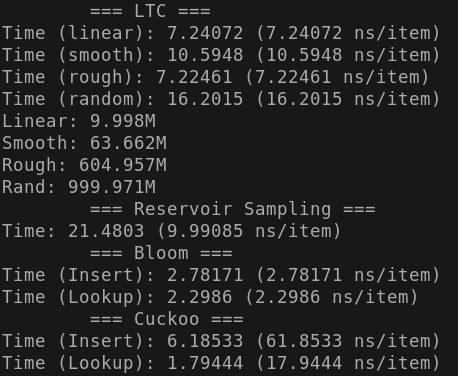
\includegraphics[width=0.25\paperwidth]{perf.png}
	\caption{Performance metric for four algorithms: LTC, Reservoir Sampling, Bloom filter and Cuckoo filter.}
	\label{fig:perf}
\end{figure}

\begin{figure}[ht]
	\begin{lstlisting}[language=C++]
	double start = When();
	for(int i = 0; i < count_add; ++i){
		bf.add(i);
	}
	double stop = When();
	\end{lstlisting}
	\caption{The performance test for adding items in the Bloom filter.
	\textbf{bf} is an instance of a Bloom filter and \textbf{count\_add} is the
	number of items to insert in the filter.}
	\label{code:perf-bloom}
\end{figure} 

\clearpage
\section{Discussion}
In conclusion, most of the project goals have been reached.  All algorithms are
independent and can be incorporated into other FreeRTOS project without
modification.  For algorithms that require specific external functions such as
memory allocation function, the library relies on templates to get the function
from the programmer.

However, this project presents many limitations that trace future work.
The performance results does not make the comparison with existing libraries presented in Section~\ref{sec:related-work}. Even though those libraries may not be comparable with the project, it would still be interesting to see their performance.
In addition to the performance metric, it should be important to have an energy consumption metric since energy efficiency is one reason of this project (Section~\ref{sec:introduction}).
Finally, it would enhance the library if both metrics were gathered on an actual sensor rather than on a laptop or on the cloud.

\bibliographystyle{plain}
\bibliography{abstract}
\end{document}
